\documentclass{article}

\usepackage{fullpage}
\usepackage{color}
\usepackage{xcolor}
\usepackage{listings}
\usepackage{array}
\usepackage{multirow}
\usepackage{footnote}
\usepackage{graphicx}

\usepackage{caption}
\DeclareCaptionFont{white}{\color{white}}
\DeclareCaptionFormat{listing}{\colorbox{gray}{\parbox{\textwidth}{#1#2#3}}}
\captionsetup[lstlisting]{format=listing,labelfont=white,textfont=white}
\lstset{
	tabsize=4,
	basicstyle=\footnotesize,
	columns=fixed,
}

\parindent0pt
\parskip10pt
\makesavenoteenv{tabular}

\title{Self Describing Wishbone Bus Specification}
\author{Manohar Vanga (BE/CO/HT)}
\begin{document}

\maketitle

\tableofcontents

\pagebreak

\section{Introduction}

This document describes the specification for the self describing Wishbone
bus.

It is advantageous from a software standpoint to have Wishbone peripherals
that can be probed automatically. This allows for a clean design of operating
system drivers.

This specification introduces a standard that allows the Wishbone bus to be
probed easily.

\pagebreak

\section{Specification}

The specification has three parts:

\begin{itemize}
\item Header block
\item ID block
\item Device descriptor block
\end{itemize}

The following points should be noted:

\begin{itemize}
\item All values are big-endian. This has been chosen as it facilitates easy
human readability of the values.
\item The presence of 64 bit registers does not imply the requirement for a
64 bit wide data bus. Multiple reads can be done using a smaller data
bus width (eg. 2 reads on a 32 bit data bus).
\end{itemize}

\subsection{Header}

The Wishbone header contains the locations of the device descriptor block and 
ID block in the Wishbone address space.

The header block can be placed anywhere within the Wishbone address space
as long as there is some way for the operating system to find its location.
It is recommended that the address of the header be placed into the configuration
space of the parent bus. For example, a BAR can be used in the case of PCI,
the CR/CSR space in the case of VME and the \emph{config} space in the case
of Etherbone.

The structure of the header block is described in Table \ref{hdr_block_struct}.

\begin{center}
	\begin{savenotes}
	\begin{table}[!ht]\footnotesize
	\caption{Wishbone header block structure}\label{hdr_block_struct}\centering
	\begin{tabular}{| c | c | c | c | c | p{5cm} |} \hline
	Offset & Size (in bytes) & Name & Access & Value & Description \\ \hline
	0x00 & 0x08 & WBHDR\_MAGIC & RO & 0x5344574248656164 & Magic number used to ensure that there is a valid header present. \\ \hline
	0x08 & 0x08 & WBIDB\_ADDR & RO & - & Address of the Wishbone ID block. See section \ref{id_block} for more information. \\ \hline
	0x10 & 0x08 & WBDDB\_ADDR & RO & - & Address of the Wishbone device descriptor block. See section \ref{device_block} for more information. \\ \hline
	\end{tabular}
	\end{table}
	\end{savenotes}
\end{center}

\begin{description}
\item[WBHDR\_MAGIC (Offset: 0x08)] \hfill \\
This field contains a unique value that allows software to ensure that
the header contains valid data. If the magic number does not match the
expected value, the software should abort immediately.

The magic number in the current version of the specification is expected to
be 0x5344574248656164 or the ASCII string "SDWBHead" without the string
terminator.

\item[WBIDB\_ADDR (Offset: 0x10)] \hfill \\
This field contains the address of the Wishbone ID block (see Section \ref{id_block}
for more information). The address width can be anything less than or equal
to 64 bits. The software reading this field should know what address width to
expect.

\item[WBDDB\_ADDR (Offset: 0x18)] \hfill \\
This field contains the address of the device descriptor block (see Section
\ref{device_block} for more information). The address width can be anything
less than or equal to 64 bits. The software reading this field should know
what address width to expect.
\end{description}

\subsection{ID Block}\label{id_block}

The ID block contains information that uniquely identifies the bitstream
within the FPGA.

The ID block additionally contains information about the parent board.
This information allows clients unable to access the parent bus memory
to know the metadata of the hardware they are accessing.

The structure of the ID block is described in Table \ref{id_block_struct}.

\begin{center}
	\begin{savenotes}
	\begin{table}[!ht]\footnotesize
	\caption{Wishbone ID block structure}\label{id_block_struct}\centering
	\begin{tabular}{| l | c | c | c | c | p{5cm} |} \hline
	Offset & Size (in bytes) & Name & Access & Value & Description \\ \hline
	0x00 & 0x08 & BSTREAM\_TYPE & RO & - & The bitstream type identifier. \\ \hline
	0x08 & 0x04 & BSTREAM\_VERSION & RO & - & The version of the specific bitstream. \\ \hline
	0x0C & 0x04 & BSTREAM\_DATE & RO & - & The synthesis date of the bitstream. \\ \hline
	0x10 & 0x14 & BSTREAM\_RELEASE & RO & - & The SVN revision number or the SHA-1 hash of the Git release. \\ \hline
	\end{tabular}
	\end{table}
	\end{savenotes}
\end{center}

\begin{description}
\item[BSTREAM\_TYPE (Offset: 0x00)] \hfill \\
The bitstream type should hold a value that uniquely identifies the type of 
bitstream present in the FPGA. Note that different bitstreams can have the
same type with differing versions (see below).

\item[BSTREAM\_VERSION (Offset: 0x08)] \hfill \\
The bitstream version should hold a value that specifies the version of the
bitstream present in the FPGA. This field along with the BSTREAM\_TYPE field,
should uniquely identify a specific bitstream.

\item[BSTREAM\_DATE (Offset: 0x0C)] \hfill \\
The bitstream date should be set to the hex-readable date of synthesis of
the bitstream. An example of a hex-readable date is 0x20111225 (25th December
2011).

\item[BSTREAM\_RELEASE (Offset: 0x10)] \hfill \\
This field should specify an identifier for the revision control software
used to manage the HDL code for the bitstream type. This allows for the 
possibility of automatic checking out and loading of bitstreams.

In the case of SVN repositories, the value of the revision number should
be stored in this field. For example, if the SVN revision is 1024, the 
stored value should be 0x00000000000000000400.

In the case of Git repositories, the 160 bit (20 bytes, 0x14 bytes) value
of the commit hash should be stored in this field.

\end{description}

\subsection{Device Descriptor Block}\label{device_block}

The device descriptor block describes all the Wishbone peripherals present
on the bus. The block is made of an array of device descriptors which have
a structure as described in Table \ref{dev_desc_struct}.

\begin{center}
	\begin{savenotes}
	\begin{table}[!ht]\footnotesize
	\caption{Wishbone device descriptor structure}\label{dev_desc_struct}\centering
	\begin{tabular}{| l | c | c | c | c | p{5cm} |} \hline
	Offset & Size (in bytes) & Name & Access & Value & Description \\ \hline
	0x00 & 0x02 & WBD\_MAGIC & RO & - & Magic number used to identify a valid device descriptor. \\ \hline
	0x02 & 0x01 & WBD\_VER\_MAJOR & RO & - & The major version of the descriptor format. \\ \hline
	0x03 & 0x01 & WBD\_VER\_MINOR & RO & - & The minor version of the descriptor format. \\ \hline
	0x04 & 0x08 & VENDOR & RO & - & The vendor ID of the vendor of the Wishbone device. \\ \hline
	0x0C & 0x04 & DEVICE & RO & - & The device ID of the Wishbone device. \\ \hline
	0x10 & 0x08 & HDL\_BASE & RO & - & Base address (Wishbone) of the Wishbone device. \\ \hline
	0x18 & 0x08 & HDL\_SIZE & RO & - & Size (in bytes) of the device address space. \\ \hline
	0x20 & 0x04 & WBD\_FLAGS & RO & - & Device flags. \\ \hline
	0x24 & 0x04 & HDL\_CLASS & RO & - & HDL class. \\ \hline
	0x28 & 0x04 & HDL\_VERSION & RO & - & HDL version. \\ \hline
	0x2C & 0x04 & HDL\_DATE & RO & - & HDL generation date. \\ \hline
	0x30 & 0x10 & VENDOR\_NAME & RO & - & Vendor name (ASCII string) \\ \hline
	0x40 & 0x10 & DEVICE\_NAME & RO & - & Device name (ASCII string) \\ \hline
	\end{tabular}
	\end{table}
	\end{savenotes}
\end{center}

\begin{description}
\item[WBD\_MAGIC (Offset: 0x00)] \hfill \\
This is a unique value used to identify a valid Wishbone device structure. If
an invalid magic value is found, it is assumed that there are no more devices
to be discovered and the auto-discovery is ended. Thus, it is used as the array
terminator for the Wishbone device block.

The magic number in all versions of the specification can be expected to
be 0x5742 or the ASCII string "WB" without the string terminator.

\item[WBD\_VER\_MAJOR (Offset: 0x02)] \hfill \\
The major version of the device descriptor format. This field is incompatible
between versions. This means that a change in the descriptor structure itself
leads to an increase in the major version. An example of a major version change
is the extension of HDL\_BASE and HDL\_SIZE to 16 bytes (128 bits).

\item[WBD\_VER\_MINOR (Offset: 0x03)] \hfill \\
The minor version of the device descriptor format. This field is compatible
between versions. This means that a change only in the minor number means the
structure is preserved. An example of a minor version change is the addition
of a new flag in the WBD\_FLAGS field.

This field and WBD\_VER\_MAJOR can be coalesced into a single WBD\_VERSION
field if needed.

\item[VENDOR (Offset: 0x04)] \hfill \\
The vendor ID of the Wishbone device. The vendor space is a 64 bit space.
The space is divided into two sections; \emph{reserved} and \emph{free}.

The \emph{reserved} vendor space includes all vendor values with the highest 
bit unset (0x0000000000000000 - 0x8FFFFFFFFFFFFFFF).

The \emph{free} vendor space includes all vendor values with the highest 
bit set (0x8000000000000000 - 0xFFFFFFFFFFFFFFFF).

Vendors are free to choose any value within the free space. There is no
guarantee of collisions of ID's with other vendors within the free space.
In the future, there could possibly be a central repository that allows
for guaranteed vendor ID's within the reserved space. The current version
of the specification however, provides no guarantee of collisions within
the reserved space. If you wish to use ID's from the reserved space, you
might need to make modifications to your device in future version of this
specification.

It is recommended that the vendor ID be chosen using an established 
hashing algorithm by feeding it uniquely identifying fields. The
recommended fields to use are the vendor name string, a 128 bit random
seed and a timestamp. It is recommended to use the MD5 hash of these
fields and take the 8 least significant bytes from the resulting hash.

\item[DEVICE (Offset: 0x0C)] \hfill \\
The device ID of the Wishbone device. Together with the vendor ID, the
device ID may be used to match device drivers. The format can be specified
in any way by a vendor as the software reading this field will be
specific to each vendor (selected based on the metadata stored in the
parent board) and is expected to know how to decode this field.

\item[HDL\_BASE (Offset: 0x10)] \hfill \\
This field contains the base address of the Wishbone device. The address width
can be anything less than or equal to 64 bits. The software reading this
field should know what address width to expect.

\item[HDL\_SIZE (Offset: 0x18)] \hfill \\
This field contains the size of the address space of this device. The address width
can be anything less than or equal to 64 bits. The software reading this
field should know what address width to expect.

\item[WBD\_FLAGS (Offset: 0x20)] \hfill \\
Currently undefined.

\item[HDL\_CLASS (Offset: 0x24)] \hfill \\
The class of the Wishbone device. The class is used to identify a device
with a specific register map, so a host driver can handle all devices of
the same class, irrespective of vendor and device numbers. This is similar
to PCI or USB devices.

\item[HDL\_VERSION (Offset: 0x28)] \hfill \\
This field specifies the version of the Wishbone device. The format can be
specified in any way by a vendor as the software reading this field will be
specific to each vendor (selected based on the metadata stored in the
parent board) and is expected to know how to decode this field.

\item[HDL\_DATE (Offset: 0x2C)] \hfill \\
The HDL date should be set to the hex-readable date of synthesis of
the Wishbone device. An example of a hex-readable date is 0x20111225 (25th
December 2011).

\item[VENDOR\_NAME (Offset: 0x30)] \hfill \\
The ASCII string representation of the vendor name. The string should be
terminated with the ASCII value 0, thus allowing for a maximum of 15
characters.

\item[DEVICE\_NAME (Offset: 0x40)] \hfill \\
The ASCII string representation of the device name. The string should be
terminated with the ASCII value 0, thus allowing for a maximum of 15
characters.
\end{description}

\section{Example Memory Map}

Figure \ref{fig:wbmap} illustrates the
structure of the Wishbone memory map for a bitstream containing three Wishbone
devices. There is a single header block that has the addresses of the other
block. There is a single ID block containing metadata regarding the bitstream
along with a single device descriptor block containing descriptors for the three
devices present in the bitstream.

\begin{figure}[!ht]
	\centering
	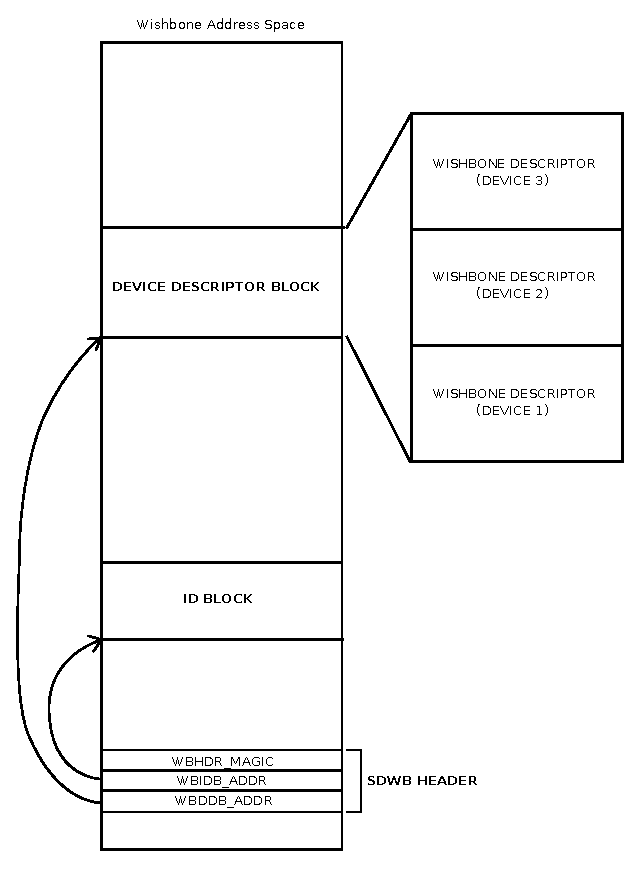
\includegraphics{wbmap.eps}
	\caption{Example memory map of a Self-Describing Wishbone bus}
	\label{fig:wbmap}
\end{figure}

\end{document}
